% Made up for the tikra benchmark.
\usetikzlibrary{shapes.symbols}
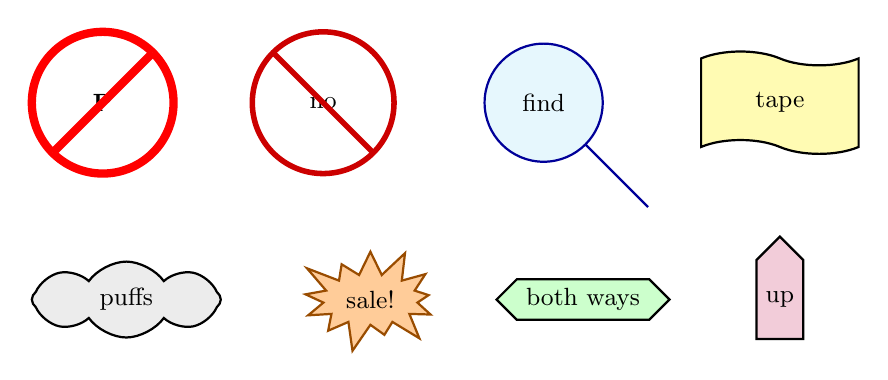
\begin{tikzpicture}[font=\small]
  \node[forbidden sign, draw=red, line width=3pt, minimum size=1.8cm, fill=white] at (0,0) {\bfseries P};
  \node[correct forbidden sign, draw=red!80!black, line width=2pt, minimum size=1.8cm] at (2.8,0) {no};
  \node[magnifying glass, draw=blue!60!black, thick, minimum size=1.5cm, fill=cyan!10] at (5.6,0) {find};
  \node[tape, draw, thick, fill=yellow!30, tape bend top=out and in, tape bend bottom=out and in, minimum width=2cm, minimum height=1.3cm] at (8.6,0) {tape};
  \node[cloud, cloud puffs=8, cloud puff arc=110, aspect=2, draw, thick, fill=gray!15, minimum width=2.4cm] at (0.3,-2.5) {puffs};
  \node[starburst, starburst points=13, starburst point height=0.4cm, draw=orange!60!black, fill=orange!40, thick] at (3.4,-2.5) {sale!};
  \node[signal, signal to=east and west, draw, fill=green!20, thick, minimum width=2cm] at (6.1,-2.5) {both ways};
  \node[signal, signal from=west, signal to=north, draw, fill=purple!20, thick, minimum height=1.3cm] at (8.6,-2.5) {up};
\end{tikzpicture}
